\documentclass[hidelinks,12pt,a4paper]{report}
\usepackage[utf8]{inputenc}
\usepackage{fontspec}
\usepackage{amsmath}
\usepackage{amsfonts}
\usepackage{amssymb}
\usepackage[margin=1in,left=1.2in,includefoot]{geometry}
% Algorithm
\usepackage{algorithm}
\usepackage{amssymb}
% IF else
\usepackage{algorithmic}
\usepackage[export]{adjustbox}
\usepackage{caption}


% Hyperlinks
\usepackage[unicode]{hyperref}
% Graphic
\usepackage{graphicx}
\usepackage{subfig}
\usepackage{float}
\renewcommand{\arraystretch}{2.5}
%----------------------------------------------------------------------------------------
%	DOCUMENT INFORMATION
%----------------------------------------------------------------------------------------

\title{}
\author{Tu \textsc{Vu}}
\date{\today}

\begin{document}

\begin{titlepage}

\includegraphics[height=1.75cm, valign=c]{images/bordeaux_logo.jpg}
\hspace*{0.3cm}
\includegraphics[height=1.75cm, valign=c]{images/LaBRI_logo.jpg}
\hspace*{1.3cm}
\includegraphics[height=1.95cm, valign=c]{images/puf_logo.jpg}\\[1.5cm]
		
	\begin{center}
	
	%\textsc{\LARGE }\\[1.5cm] % Main heading such as the name of your university/college
	
	\textsc{\Large UNIVERSITY OF BORDEAUX}\\[1.5cm] % Major heading such as course name
	
	\textsc{\large INTERNSHIP REPORT}\\[1.5cm] % Minor heading such as course title


%{\large Final report}\\[0.5cm]	
	
	\line(1,0){400}\\[0.2in]
	\huge{\bfseries Deep Learning \\ Image Classification}\\
	\line(1,0){400}\\[1.5cm]
	\noindent	
	\begin{minipage}{0.4\textwidth}
		\begin{flushleft} \large
    	\emph{Student:}\\
    	Manh Tu \textsc{Vu}
		\end{flushleft}
	\end{minipage}
	\begin{minipage}{0.4\textwidth}
  		\begin{flushright} \large
    		\emph{Supervisor:} \\
    		Marie \textsc{Beurton-Aimar}
    		Van Linh \textsc{Le}
  		\end{flushright}
	\end{minipage}
	
	\vfill

% Bottom of the page
{\large \today}
	\end{center}
\end{titlepage}

\chapter*{Acknowledgements}

First of all, I would like to express my deepest gratitude to my two supervisors, Mrs. Marie BEURTON-AIMAR and Mr. Van Linh LE for their agreements, guide, and support during the planning and developing of my internship.
\\
\\
I would like to thank Mr Fabien BALDACCI for his generous help and comment during my work. I would like to thank the staffs, students in LaBRI, who helped, supported with the technique and providing me a professional working environment.
\\
\\
I would also like to thank all the professors in the University of Bordeaux and the PUF-HCM, who imparted a lot of knowledge about learning and researching. Finally, I would like to thank my family and colleagues for their support and encouragement through my study.

\clearpage

\chapter*{Abstract}

Deep Learning is a subfield of machine learning concerned with algorithms inspired by the structure and function of the brain called artificial neural networks.
\\
\\
Image classification is a field that has many applications in life. It could be useful to categorize images, provide only images which the user are interesting, protect the children from unwanted contents such as violent or sexual. 
\\
\\
Although it already has a lot of algorithms to solve the Image classification problem. However, those (algorithms) are hard to implement and just specific to some domains. With the advent of deep learning, this problem become more easier and obtained a high performance result\cite{o.a.b.penattik.nogueiraj.a.dossantos2015}.
\\
\\
The goal of my internship at LaBRI is research \& implement the Deep learning in Image classification to classify images from \href{https://heobs.org}{heobs.org}. Try to do in different approach, compare them and finally, choose the one which give the best result.
% Table content
\tableofcontents
\listoffigures
\thispagestyle{empty}
\clearpage

\chapter*{Introduction}
Heritage Observatory project has for aim to identify cultural and historical heritages, constitute a specific database, provide a data archive free for all. This platform allows us to receive the breaking news about cultural or historical heritage sites located in regions of the world that we are interesting. In order to do that, the platform will collect a huge of images about the cultural and historical heritage. The problem appears when we want to categorize those images into a specific classes when the image have no label and we can't looking to each of those images and categorize it by hand. We need to find a way to let the computer do it for us.
The aim of my internship is to implement a deep-learning algorithm to classify those images.
\\
\\
Image classification is the task of assigning an input image one label from a fixed set of categories. There are lots of classifiers that exists, but nowadays, neural networks and deep learning currently provide the best solutions to many problems in image and speech recognition, and in natural language processing.
\\
\\
Deep learning, is a part of machine learning and it gives techniques for learning in neural networks. Neural networks are inspired by the human system of neurons that is able to learn from observations. It is feed by labeled data and learns automatically from that. The most adapted neural network for image recognition is the convolutional neural network (CNN). It's adapted to the recognition of 4 classes: being, heritage, scenery and other. That's why it has been implanted.
\\
\\
Deep learning has two major categories of image classification techniques include unsupervised and supervised classification. With unsupervised classification, all images are unlabeled and we using deep learning to learn to inherent structure from the image input data while with supervised classification, all images are labeled and we using deep learning to learn to predict the output from the image input data.
\\
In this project, we'll implement both of those categories of image classification techniques and then compare the result to see which one are better to solve our problem.
\chapter{Context}
\section{Pôle Universitaire Français}
The Pôle Universitaire Français (PUF) was created by the intergovernmental agreement of VietNam and France in October 2004. With ambition is building a linking program between the universities in VietNam and the advanced programs of universities in France. There are two PUF’s center in VietNam: Pôle Universitaire Français de l’Universite Nationalé du Vietnam - Ha Noi located in Ha Noi capital (PUF-Ha Noi) and Pôle Universitaire Français de l’Universite Nationalé du Vietnam - Ho Chi Minh Ville located in Ho Chi Minh city (PUF-HCM).
\subsection{PUF-HCM}
PUF-HCM\footnote{\url{http://pufhcm.edu.vn}} is a department of VietNam National Univeristy at Ho Chi Minh city. From the first year of operations, PUF-HCM launched the quality training programs from France in VietNam. With target, bring the programs which designed and evaluated by the international standards for Vietnamese student. PUF-HCM always strive in our training work. So far, PUF-HCM have five linking programs with the universities in France, and the programs are organized into the subjects: Commerce, Economic, Management and Informatics. In detail:

\begin{itemize}
	\item Bachelor and Master of Economics : linking program with University of Toulouse 1 Captiole
	\item Bachelor and Master of Informatics: linking program with University of Bordeaux and University of Paris 6.
\end{itemize}
The courses in PUF-HCM are provided in French, English and Vietnamese by both Vietnamese and French professors. The highlight of the programs are inspection and diploma was done by the French universities.
\section{Laboratoire Bordelais de Recherche en Informatique}
The Laboratoire Bordelais de Recherche en Informatique (LaBRI)\footnote{\url{http://www.labri.fr}} is a research unit associated with the CNRS (URM 5800), the University of Bordeaux and the Bordeaux INP. Since 2002, it has been the partner of Inria. It has significantly increased in staff numbers over recent years.
In March 2015, it had a total of 320 members including 113 teaching/research staff (University of Bordeaux and Bordeaux INP), 37 research staff (CNRS and Inria), 22 administrative and technical (University of Bordeaux, Bordeaux INP, CNRS and Inria) and more than 140 doctoral
students and post-docs. The LaBRI’s missions are: research (pure and applied), technology application and transfer and training.
Today the members of the laboratory are grouped in six teams, each one combining basic research, applied research and technology transfer:
\begin{itemize}
	\item Combinatorics and Algorithmic
	\item Image and Sound
	\item Formal Methods
	\item Models and Algorithms for Bio-informatics and Data Visualisation
	\item Programming, Networks and Systems
	\item Supports and Algorithms for High Performance Numerical Applications
\end{itemize}
Within these team, research activities are conducted in partnership with Inria. Besides that, LaBRI also collaborate with many other laboratories and companies on French, European and the international.
\newpage
\section{The internship project: Deep Learning Image Classification}

The internship is intended to be a duration to apply the knowledge to the real environment. It shows the ability synthesis, evaluation and self-research of student. Besides, the student may study the experience from the real working environment. My internship is done under the
guidance of Mrs Marie BEURTON-AIMAR in a period of six months at LaBRI laboratory.
The project is working on the Image Classification field. The goal of the project is using Deep Learning to classify all images from \href{https://heobs.org}{https://heobs.org} into 4 classes, include:
\begin{description}
\item[Heritage] \hfill \\ A place of cultural, historical, or natural significance for a group or society.
\item[Beings] \hfill \\ Any form of life, such as a plant or a living creature, whether human or other animal.
\item[Scenery] \hfill \\ Any form of landscapes which show little or no human activity and are created in the pursuit of a pure, unsullied depiction of nature, also known as scenery.
\item[Other] \hfill \\ Any other type of image that doesn't represent a photograph, such as painting, illustration, any object.	
\end{description}
The administrator of \href{https://heobs.org}{https://heobs.org} has collected a set of 144564 images about vietnamese human, statue, ancient artifacts, building, landscape, etc. But all of them are completed unlabeled. So, the question is: ``How we can classify those images to the right classes and how to automatic classify the new image, which the machine has never seen to the right class''.\\
The objective of this internship is implementing a method to automatic classify images.
The method is use deep convolutional neural networks (CNNs or ConvNets) to tackle the remote sensing scene classification task.
\newpage
\begin{figure}[!htb]
\subfloat[]{%
\begin{minipage}{\linewidth}
  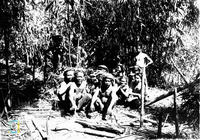
\includegraphics[width=5cm, height=3.5cm]{images/sample/being_6}\hfill
  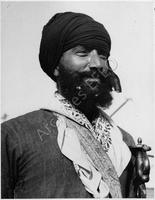
\includegraphics[height=3.5cm]{images/sample/being_35}\hfill
  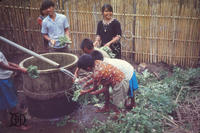
\includegraphics[width=5cm, height=3.5cm]{images/sample/being_45}%
\end{minipage}%
}\par
\subfloat[]{%
\begin{minipage}{\linewidth}
  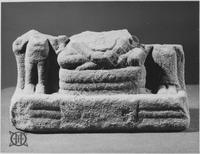
\includegraphics[width=5cm, height=3.5cm]{images/sample/heritage_145}\hfill
  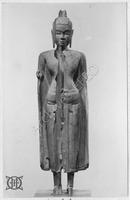
\includegraphics[height=3.5cm]{images/sample/heritage_147}\hfill
  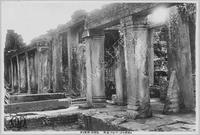
\includegraphics[width=5cm, height=3.5cm]{images/sample/heritage_282}%
\end{minipage}%
}\par
\subfloat[]{%
\begin{minipage}{\linewidth}
  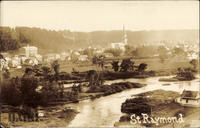
\includegraphics[height=2.8cm]{images/sample/scenery_111}\hfill
  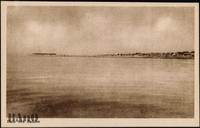
\includegraphics[height=2.8cm]{images/sample/scenery_102}\hfill
  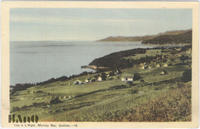
\includegraphics[height=2.8cm]{images/sample/scenery_110}%
\end{minipage}%
}\par
\subfloat[]{%
\begin{minipage}{\linewidth}
  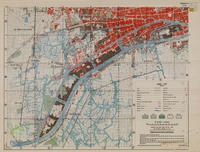
\includegraphics[width=5cm, height=3.5cm]{images/sample/other_129}\hfill
  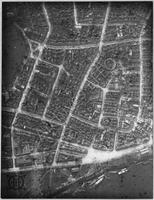
\includegraphics[height=3.5cm]{images/sample/other_190}\hfill
  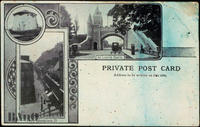
\includegraphics[width=5cm, height=3.5cm]{images/sample/other_202}%
\end{minipage}%
}
  \caption{Images from heobs.org}
\end{figure}

\chapter{Methods to solve our problem}
In this part, we will explain how we choose the aglorithms to solve our problem and describe what is each one.
\section{Scikit-learn algorithm cheat-sheet\cite{scikitlearn.org}}
Because it has many algorithms has able to classify images such as: Decision tree\cite{j.r.quinlan1985}, SVM\cite{stever.gunn1998}, K-nearest neighbors\cite{orenanavakfiry.levy2017}, etc. We need to find a right one to solve our problem. The Scikit-learn had made an algorithm cheat-sheet to help us to choose the right one:

\begin{figure}[ht]
	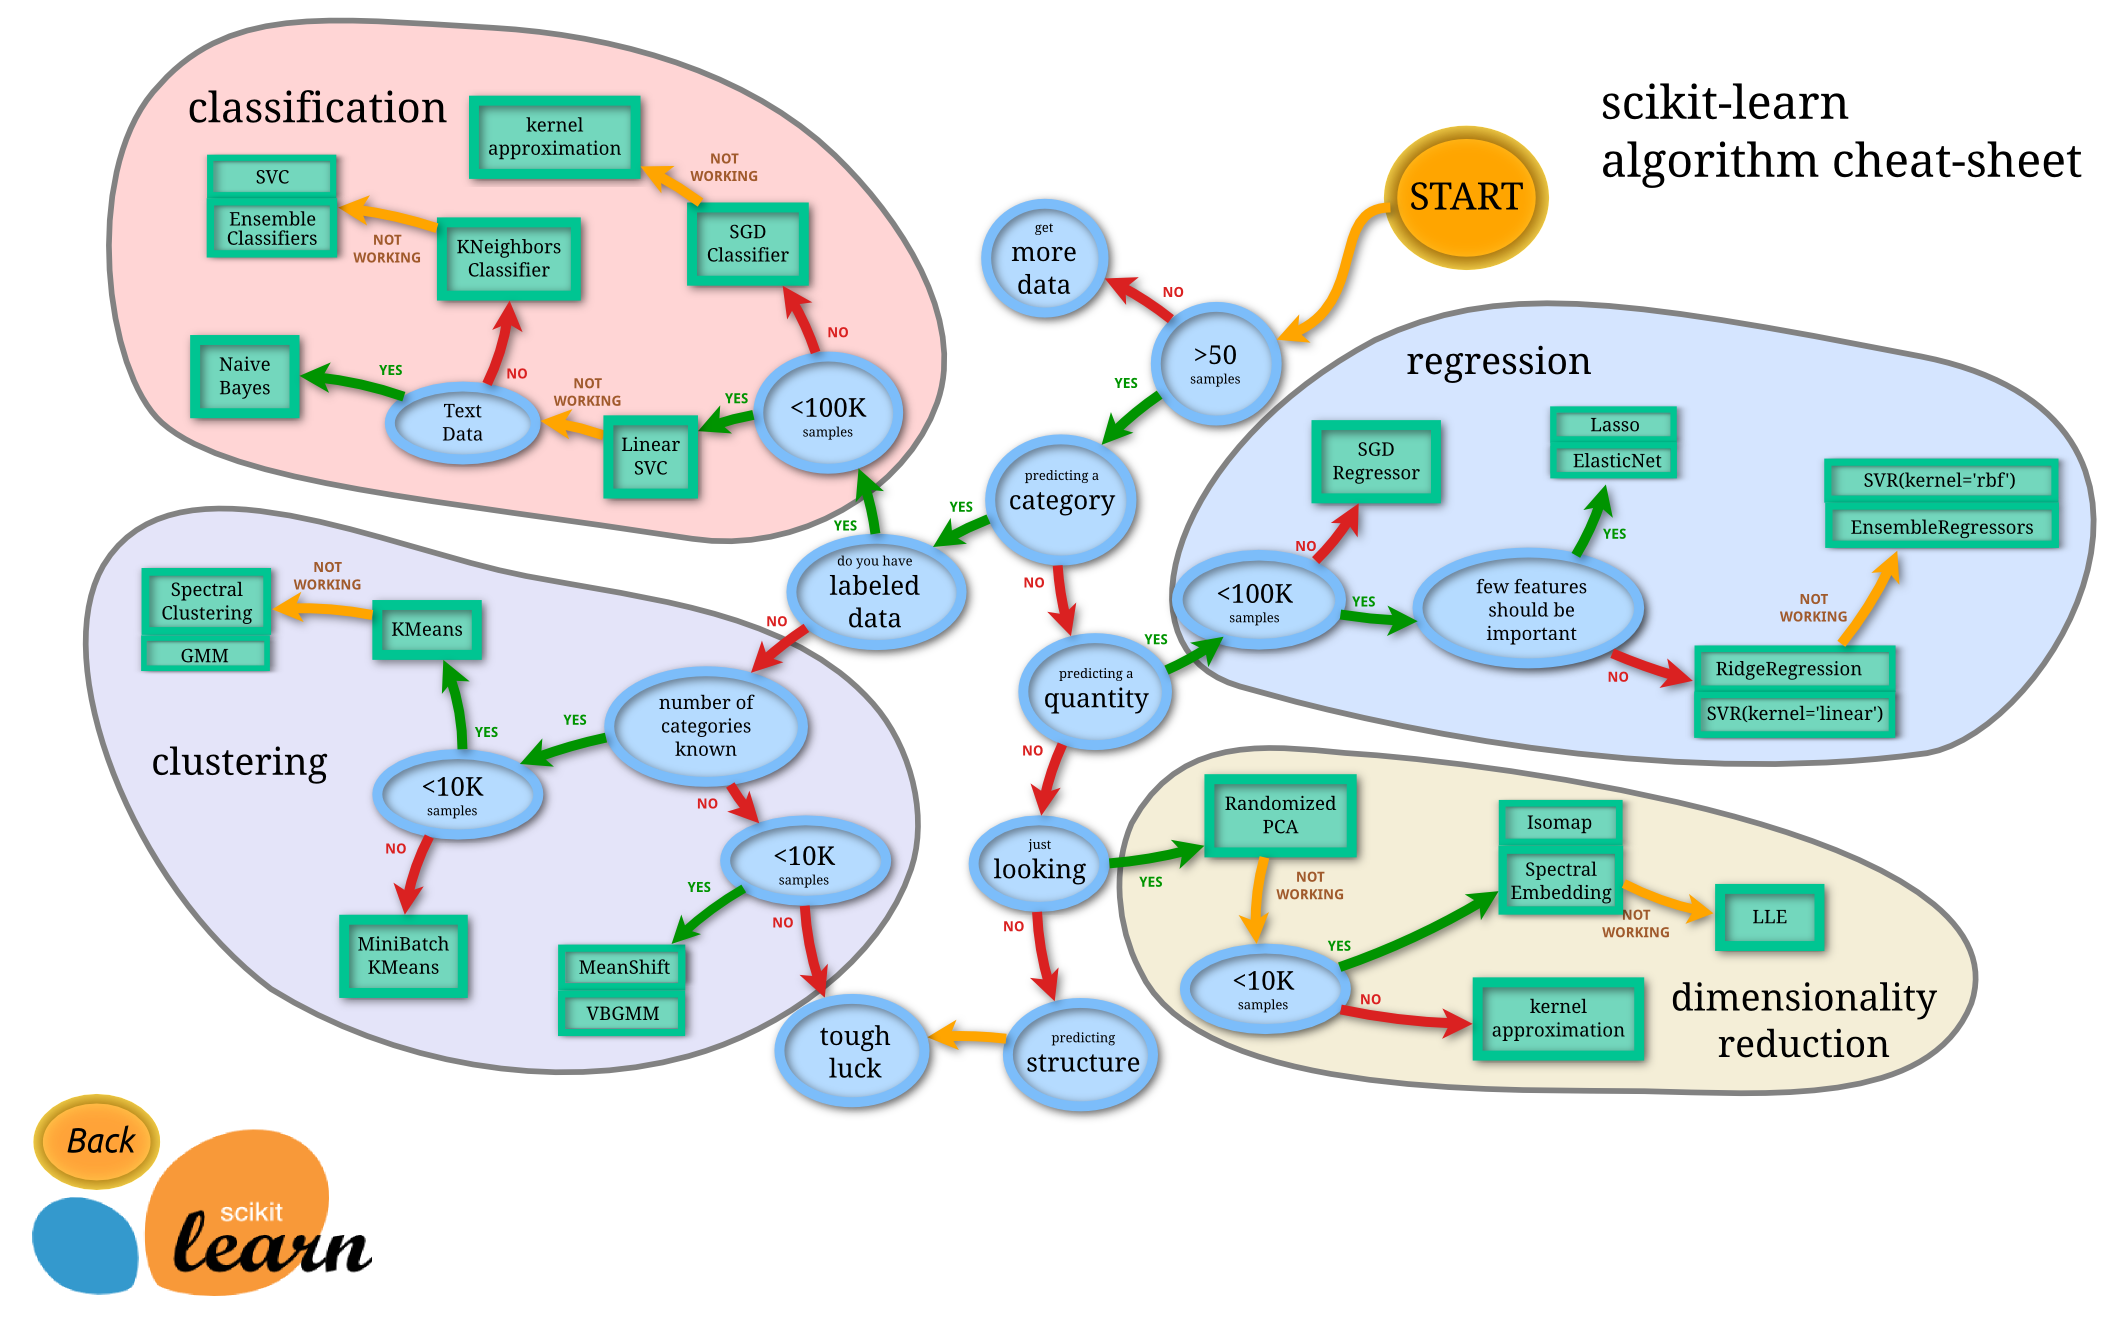
\includegraphics[width=\textwidth, center]{images/scikit-learn}
	\caption{Scikit-learn algorithm cheat-sheet}
	\label{fig:Scikit-learn}
\end{figure}
This algorithm cheat-sheet(see Fig \ref{fig:Scikit-learn}) suggests to use K-mean algorithm to classify our images because of unlabeled images and, the size of our dataset is less than 10K samples. However, one can note that it is mandatory to create a labeled dataset from our unlabeled images by hand and then, we can use SGD Classifier to do it.
\\
Finally, two ways are proposed to reach our goal: one is use Supervised Classification with SGD is our main algorithm. The other is use Unsupervised Classification with K-mean is main algorithm. Both of them can be applied by using Convolution Neural Network(CNN).
\section{General CNN architecture}
A convolutional network is a neural network that use convolutions. It is a multiplayer network (e. g. it uses several layers). In reality, those kind of network, are dividing in two part. The first one use convolutional layers - layers that use convolution patches to compute weights used in neurons. The second part, used to connect the first part to the output, is made of fully connected layers: every output of a layer is connected to every neurons of the next one without any distinctions.

\begin{figure}[ht]
	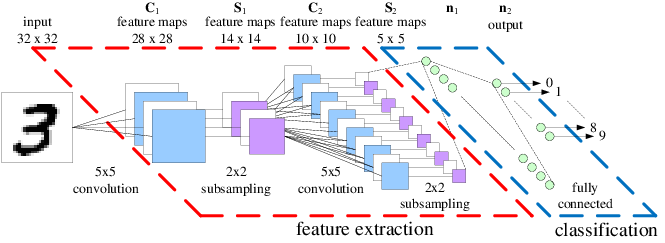
\includegraphics[scale=1, center]{images/Fig-1-An-Example-CNN-architecture-for-a-handwritten-digit-recognition-task}
	\caption{An Example CNN architecture for a handwritten digit recognition task.}
	\label{fig:CNN-architecture}
\end{figure}
The network architecture of an example CNN is depicted in Fig \ref{fig:CNN-architecture}. The processing starts with feature extraction layers and is finished by fully connected classification layers. Using different layers delivers robust recognition accuracy and is invariant to small geometric transformations of the input images. The robust recognition accuracy makes that CNN are successfully used for classification tasks on real world data

\section{Libraries}
The fact is, we're unable to do eveything from scratch, CNN's too complex if we want to build it by our self. There have a several libraries for CNN, which developed by some companies, universities or researching labs to help us to make easy to construct and configure our model. Below is some of those libraries:
\begin{itemize}
	\item \textbf{Caffe}\footnote{\url{http://caffe.berkeleyvision.org}} a deep learning framework made with expression, speed, and modularity in mind.
	\item \textbf{Tensorflow}\footnote{\url{https://www.tensorflow.org}} an open source software library for numerical computation using data flow graphs.
	\item \textbf{Theano}\footnote{\url{http://deeplearning.net/software/theano}} CPU/GPU symbolic expression compiler in python (from MILA lab at University of Montreal)
	\item \textbf{Keras}\footnote{\url{https://keras.io}} a high-level neural networks API, written in Python and capable of running on top of TensorFlow, CNTK, or Theano.
	\item \textbf{Torch}\footnote{\url{http://torch.ch}} a scientific computing framework with wide support for machine learning algorithms that puts GPUs first. 
\end{itemize}

And much more other libraries. So, It’ll be hard to know that which one is the best. However, we all know that they will do well their job. The thing most important here is the network model and the configure parameters. \\
\\
So, after some researched, we found many papers, articles relevance with our problem such as: \cite{placesdatabase}, \cite{landclassification}. They implemented Caffe Library. So, we choose \textbf{Caffe} as our library to represent the CNN model since it’s one of the most popular libraries for deep learning (convolutional neural networks in particular). It's developed by the Berkeley Vision and Learning Center (BVLC) and
community contributors. It’s easily customizable through configuration files, easily extendible with new layer types,
and provides a very fast ConvNet implementation (leveraging GPUs, if present). It provides C++, Python and MATLAB APIs.

\section{The ImageNet Visual Recognition Challenge}

The ImageNet Visual Recognition Challenge\footnote{\url{http://www.image-net.org/challenges/LSVRC/2012}} is a competition where research teams evaluate their algorithms on the given data set, and compete to achieve higher accuracy on several visual recognition tasks such as Classification, Classification with localization or Fine-grained classification. \\
Because they have the same kind of goal with our project, so, we will try to implement the CNN model of the winner of this challenge and also try to improve it to get the better result.

\chapter{The Dataset}
Because both Supervised and Unsupervised Classification are required dataset to train and test, this chapter describes how we obtain the dataset and optimize it.
\section{Fetch all images}
The entire image dataset described on the text file named ”photos.txt” line by line. Each line includes the image id and image description as below:
\begin{verbatim}
5a36f382-dbdf-11e6-95fd-d746d863c3eb | Những người ăn xin  | vie
5a36f382-dbdf-11e6-95fd-d746d863c3eb | Mendiants  | fra
17be8122-dbe0-11e6-860c-5fea02802d0a | Chợ Cũ (3) | vie
17be8122-dbe0-11e6-860c-5fea02802d0a | Vieux marché (3) | fra
400286c8-dbe1-11e6-bb4d-ff975c68de04 | Ngân hàng Đông Dương  | vie
400286c8-dbe1-11e6-bb4d-ff975c68de04 | La Banque de l’Indochine  | fra
\end{verbatim}
In order to get the image dataset, we have to fetch each image one by one by join the image id with heobs cdn url \href{https://cdn.heobs.org/photo/}{https://cdn.heobs.org/photo/}. For example, with the first line in the record above, we have the following URL: 
\begin{verbatim}
https://cdn.heobs.org/photo/5a36f382-dbdf-11e6-95fd-d746d863c3eb
\end{verbatim}
We wrote a small python script to automatic read this text file \& download images one by one.
Totally, we have 142459 images in our dataset.

\section{Remove broken images}
After downloaded \& look around all images, we found that it has a lot of broken images, which can't be displayable. So, we write a python script to filter all of those broken images automatically. \newline
Finally, we have 89850 images left in our dataset.

\section{Labeling image dataset}
It's mandatory to label our images for both Supervised and Unsupervised Classification because with Unsupervised Classification, we need a labeled dataset to validate if the image is classified correct or not. With Supervised Classification, we need a labeled dataset to train \& validate the Neural Network Model.\newline\newline
Because our images have different resolution, so, to build a good dataset, we loop through all our images and find all images, which has the most common image resolution, keep all those images and reject all others.


\chapter{Unsuppervised Deep Learning}
\chapter{Suppervised Deep Learning}

\bibliographystyle{ieeetr}
\bibliography{bibfile}
\end{document}